\documentclass[a4paper,12pt]{article}

\usepackage{oeNIKstyle}

%% Írd át a saját adataidra!
\author{Gipsz Jakab}
\torzsKonyvSzam{1234567/123}

%% Bibliográfia stílus definíció, váltohat..
\bibliographystyle{IEEEtrans}

\begin{document}

\makepreamble

% A szövegtörzset célszerű több fájlba bontani, mindet külön külön be lehet húzni a kövektező módon: (Lehetőleg sectionönként, nem úgy ahogy az example-ben van ömlesztve)
%Példa az alapvető parancsok használatára
\section{Összefoglaló}

A példa röviden összefoglalja a reportok írásához a jelen sablon használatát és a benne foglalt speciális parancsokat.

\subsection{Szöveg}
\lipsum

\section{Ábrák beszúrása}\label{sec:figures}

Example for figures: see figure \ref{fig:neuron} with footnote citation

\begin{figure}[H]
    \centering
    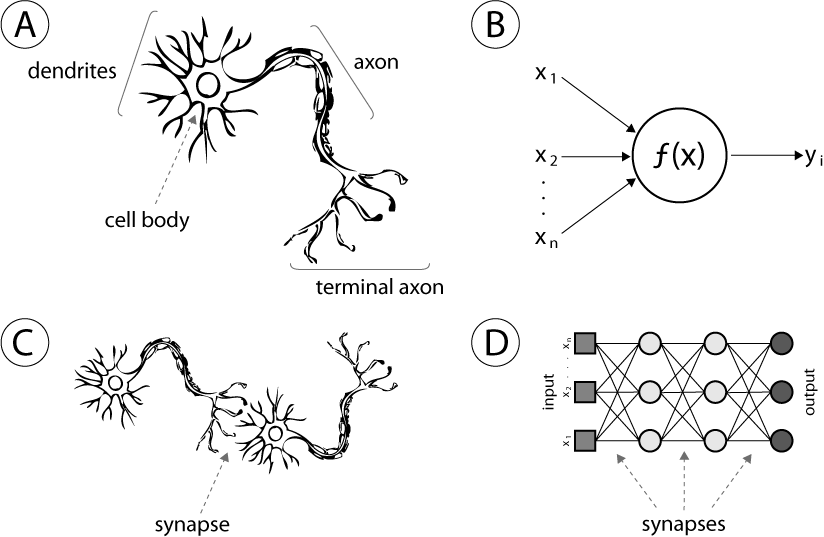
\includegraphics[width=\textwidth]{img/neuron.png}
    \caption[Biological and artificial neurons and neural networks]{\centering Biological and artificial neurons and neural networks\footnotemark \newline (A) biological neuron, (B) artificial neuron, (C) connection of biological neurons, (D) connection of artificial neurons (ANN) \newline
    See more information in \cite{goodfellow_deep_learning}}
    \label{fig:neuron}
\end{figure}


\footnotetext{\url{http://www.intechopen.com/source/html/39067/media/image1.png}}

\section{Linkek beszúrása}\label{sec:links}

Példa linkre: \href{https://www.youtube.com/watch?v=VQS4uUtm2kw}{\texttt{https://www.youtube.com/watch?v=VQS4uUtm2kw}}.

\pagebreak
\section{Kód beszúrása}
Külön fájlból:
\lstinputlisting[language=C++]{"codes/code_example.txt"}

Inline:
%Node the indentation with spaces not tabs
\begin{verbatim}
class BankAccount(object):
  def __init__(self, initial_balance=0):
    self.balance = initial_balance
  def deposit(self, amount):
    self.balance += amount
  def withdraw(self, amount):
    self.balance -= amount
  def overdrawn(self):
    return self.balance < 0
my_account = BankAccount(15)
my_account.withdraw(5)
print my_account.balance
\end{verbatim}

\pagebreak



\bibliography{bibliography}
\end{document}
